% !TeX spellcheck = it_IT
% !TXS template
\documentclass[italian]{article}
\usepackage[T1]{fontenc}
\usepackage[utf8]{inputenc}
\usepackage{lmodern}
\usepackage[a4paper,top=3cm,bottom=3cm,left=2.5cm,right=2.5cm]{geometry}
\usepackage[italian]{babel}
\usepackage{enumitem}
\usepackage[fleqn]{amsmath}
\usepackage{amssymb}
\usepackage{mathtools}% http://ctan.org/pkg/mathtools
\usepackage{cancel}
\usepackage{color}
\usepackage[usenames,dvipsnames]{xcolor}
\usepackage{units}
\usepackage{hyperref}
\usepackage{textcomp}
\usepackage{soul}
\usepackage{listings}
\usepackage{pifont} %https://www.rpi.edu/dept/arc/training/latex/LaTeX_symbols.pdf
\usepackage{fontspec}
\usepackage{fontawesome}
\usepackage{mdframed}
\usepackage{pgf,tikz}
\usepackage{mathrsfs}
\usetikzlibrary{arrows}
\usepackage{multicol}
\usepackage{titlesec}
\usepackage{inconsolata}

\hypersetup{
	colorlinks,
	citecolor=black,
	filecolor=black,
	linkcolor=black,
	urlcolor=blue
}


%% PHP
\definecolor{dkgreen}{rgb}{0,.6,0}
\definecolor{dkblue}{rgb}{0,0,.6}
\definecolor{dkyellow}{cmyk}{0,0,.8,.3}

\lstset{
	language = php,
	basicstyle=\small\ttfamily,
	numbers=left,
	numberstyle=\scriptsize,
	stepnumber=1,
	numbersep=8pt,
	showstringspaces=false,
	breaklines=true,
	frame=lines,
	backgroundcolor=\color{background},
	keywordstyle    = \color{dkblue},
	stringstyle     = \color{red},
	identifierstyle = \color{dkgreen},
	commentstyle    = \color{gray},
	emph            =[1]{php},
	emphstyle       =[1]\color{black},
	emph            =[2]{if,and,or,else},
	emphstyle       =[2]\color{dkyellow}
}

%% JSON
\colorlet{punct}{red!60!black}
\definecolor{background}{HTML}{EEEEEE}
\definecolor{delim}{RGB}{20,105,176}
\colorlet{numb}{magenta!60!black}

\lstdefinelanguage{json}{
	basicstyle=\normalfont\ttfamily,
	numbers=left,
	numberstyle=\scriptsize,
	stepnumber=1,
	numbersep=8pt,
	showstringspaces=false,
	breaklines=true,
	frame=lines,
	backgroundcolor=\color{background},
	literate=
	*{0}{{{\color{numb}0}}}{1}
	{1}{{{\color{numb}1}}}{1}
	{2}{{{\color{numb}2}}}{1}
	{3}{{{\color{numb}3}}}{1}
	{4}{{{\color{numb}4}}}{1}
	{5}{{{\color{numb}5}}}{1}
	{6}{{{\color{numb}6}}}{1}
	{7}{{{\color{numb}7}}}{1}
	{8}{{{\color{numb}8}}}{1}
	{9}{{{\color{numb}9}}}{1}
	{:}{{{\color{punct}{:}}}}{1}
	{,}{{{\color{punct}{,}}}}{1}
	{\{}{{{\color{delim}{\{}}}}{1}
	{\}}{{{\color{delim}{\}}}}}{1}
	{[}{{{\color{delim}{[}}}}{1}
	{]}{{{\color{delim}{]}}}}{1},
}


\author{
	Giacomo De Liberali - 857174\\
	Daniele Rigon - 857319 \\
	Denny Ruffato - 859171 \\
	Luca Fortin - 858986
}

\begin{document}
	
\title{Base di Dati - Relazione}
\maketitle

\tableofcontents
\pagebreak

\section{Introduzione}
L’applicazione, reperibile \href{http://wwwstud.dsi.unive.it/druffato/bd2017/}{qui}, è un forum di recensione libri composta da un insieme di pagine dinamiche sviluppate in \textit{PHP} e un database \textit{postgreSQL}. L'utente, una volta registratosi, potrà usufruire del catalogo, integrarlo con nuovi dati e fornire recensioni e commenti. \\\\

\noindent
L'applicazione permette le seguenti operazioni:
\begin{itemize}
	\item Visualizzazione catalogo libri
	\item Visualizzazione dettaglio di un libro con le recensioni e commenti
	\item Aggiunta di una recensione per ogni libro
	\item Aggiunta di commenti ad una recensione
	\item Aggiunta di commenti di risposta ad un altro commento
	\item Aggiunta di un giudizio positivo/negativo a commenti e/o recensioni
	\item Ordinamento del catalogo libri per giudizio positivo crescente/decrescente
	\item Registrazione di un nuovo utente
	\item Possibilità di Login e Logout
\end{itemize}
\section{Progetto e funzionalità}
\subsection{Homepage}
La pagina iniziale, visualizzabile solamente dopo aver effettuato il login, permette di visualizzare il catalogo dei libri in modo ordinato.
In questa pagina si possono ordinare i libri in base al giudizio e ricercarli per titolo o autore.

\subsection{Login}
Questa pagina, composta da un semplice form a due input, permette ad un utente già registrato di accedere al portale e di visualizzare, quindi, il catalogo.

\subsection{Logout}
La funzione di logout è permessa solo da utenti registrati e autenticati al sito.
Quando l’utente vorrà scollegarsi dal sito cliccherà sulla voce “Logout” presente nella navbar e sarà disconnesso senza ulteriori richieste. Dopo essersi disconnesso, sarà possibile autenticarsi con un altro profilo.

\subsection{Registrazione}
Un utente può registrarsi al sito compilando il form proposto, scegliendo anche il proprio username e la propria password, oltre alle informazioni personali quali nome, cognome, email e data di nascita. L'email viene inserita, sebbene non riporti utilità per questo progetto, per eventuali sviluppi futuri dell'applicazione. Dopo aver inserito le informazioni richieste l'utente dovrà cliccare sul bottone per registrarsi e, se le informazioni sono corrette (ovvero l’username scelto non appartiene ad un altro utente) allora l'utente sarà inserito nel database.
Dopo essersi registrato, sarà possibile effettuare il login inserendo le nuove credenziali.

\subsection{Ricerca di un libro}
Un utente può cercare libri o autori nel database tramite l’area di ricerca posta nella navbar in alto a destra, che rimanderà nella homepage con i soli risultati filtrati.
A questo punto è possibile cliccare sul libro cercato (se presente nel database) per visualizzare la scheda del libro, con le informazioni su di esso ed eventuali recensioni e commenti.

\subsection{Inserire un libro}
Se l'utente è autenticato viene permesso di inserire un libro. Cliccando su “Add book”, presente nella navbar, si viene reindirizzati ad una pagina contenente un form da completare con le informazioni del libro: titolo, autore, genere e immagine.

\subsection{Inserire un autore}
Se l'utente è autenticato viene permesso di inserire un autore, il quale sarà poi disponibile nel form di aggiunta libro. Cliccando su “Add author”, presente nella navbar, si viene reindirizzati ad una pagina contenente un form da completare con le informazioni dell’autore: nome, cognome, data di nascita e nazionalità

\subsection{Recensire un libro}
Ogni utente può aggiungere una nuova recensione ad un libro, la quale può essere votata e commentata. Ogni utente può votare "Up" o "Down" la recensione, e togliere il proprio voto se necessario. Un contatore sarà aumentato e decrementato, tenendo così conto dei voti dati fino a quel momento. 

\subsection{Commentare una recensione e/o un commento}
Sotto ogni recensione e ogni commento è possibile aggiungere un nuovo commento.

\subsection{Votare commenti e recensioni}
Ogni recensione e ogni commento possono essere votati con un voto "Up" o "Down".

\pagebreak
\section{Sitemap}
La seguente immagine rappresenta la struttura del sito e la sua navigazione.
\begin{figure}[h]
	\centering
	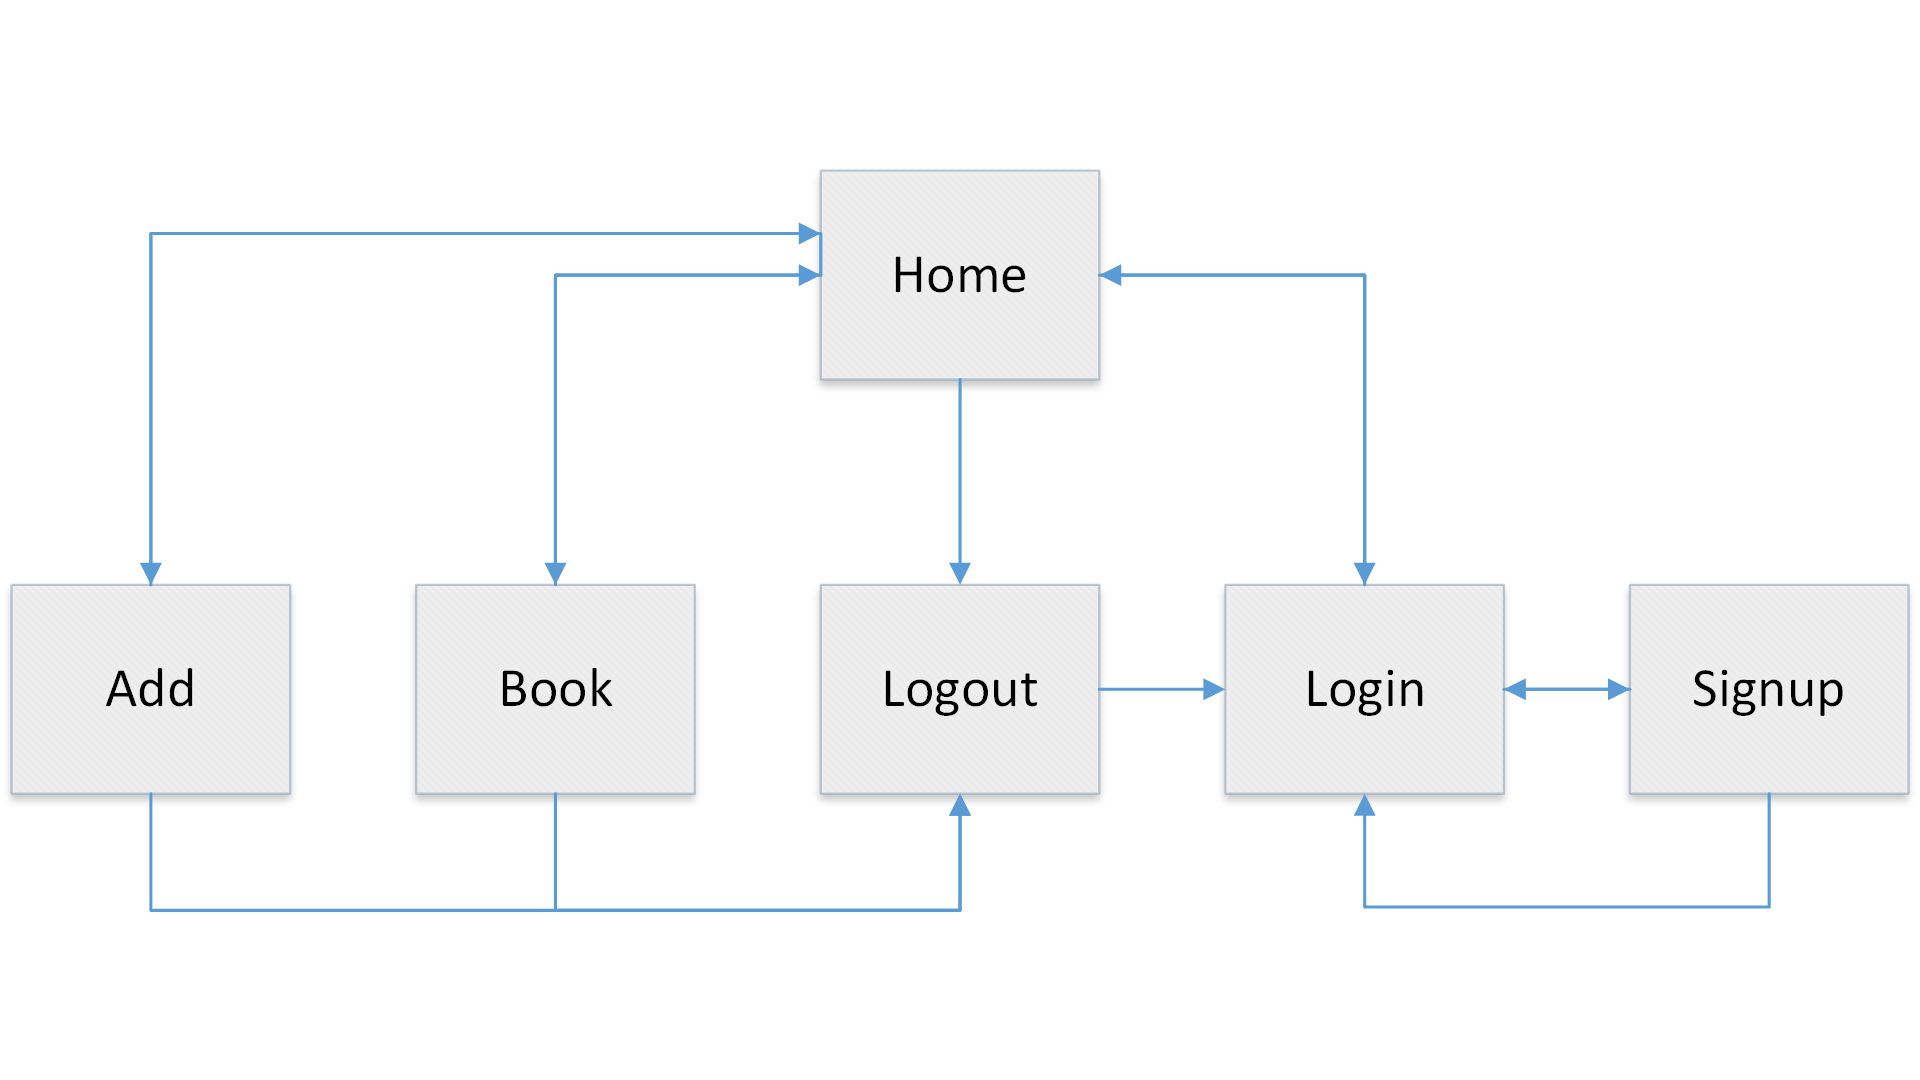
\includegraphics[width=1\linewidth]{images/sitemap}
	\caption[Sitemap]{Struttura di navigazione del portale}
	\label{fig:sitemap}
\end{figure}

\pagebreak
\section{Database}
\subsection{Modello concettuale}
\begin{figure}[h]
	\centering
	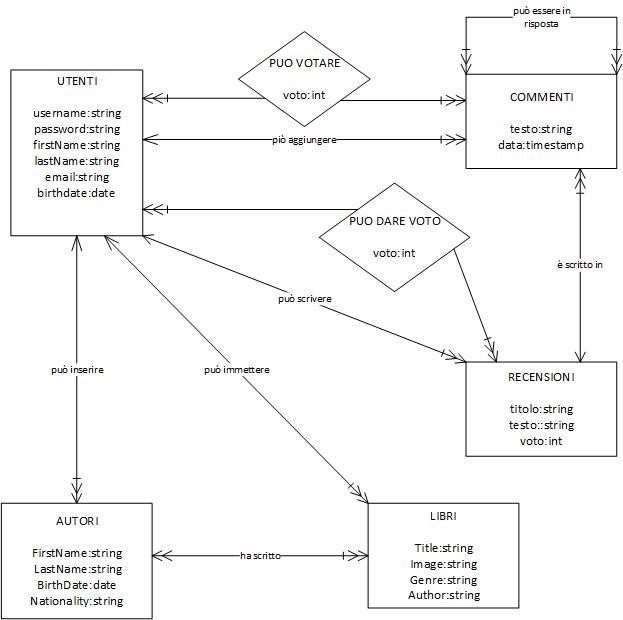
\includegraphics[width=1\linewidth]{images/schema_concettuale}
	\caption[Schema concettuale]{Schema concettuale del database dell'applicazione.}
	\label{fig:schemaconcettuale}
\end{figure}
\pagebreak
\subsection{Modello relazionale}
\begin{figure}[h]
	\centering
	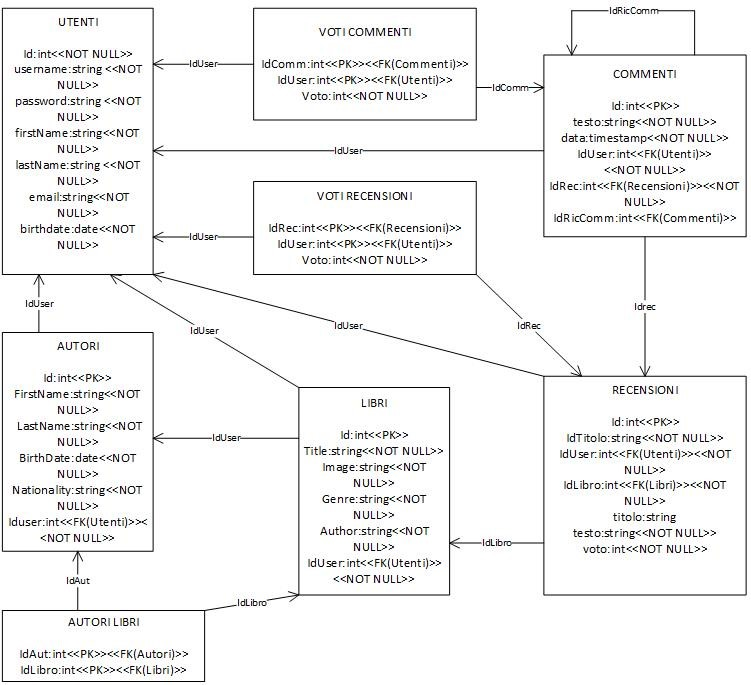
\includegraphics[width=1\linewidth]{images/schema_relazionale}
	\caption[Schema relazionale]{Schema relazionale del database dell'applicazione.}
	\label{fig:schemarelazionale}
\end{figure}
\pagebreak
\section{Codice}
Sarà presentato di seguito il codice dell'intera applicazione, suddiviso per responsabilità.


\subsection{Models}
Tutti i file in questa sezioni sono nella directory \textit{/php/models} e rappresentano i modelli dei dati, nonché delle tabelle del database.

\subsubsection{DatabaseConnection.php}
Rappresenta una connessione al database.
\lstinputlisting{../php/models/DatabaseConnection.php}

\subsubsection{Author.php}
Rappresenta un autore di libri.
\lstinputlisting{../php/models/Author.php}

\subsubsection{Book.php}
Rappresenta un libro scritto da un autore.
\lstinputlisting{../php/models/Book.php}

\subsubsection{Review.php}
Rappresenta una recensione di un libro da parte di un utente.
\lstinputlisting{../php/models/Review.php}

\subsubsection{Comment.php}
Rappresenta un commento ad una recensione od ad un altro commento scritto da un utente.
\lstinputlisting{../php/models/Comment.php}

\subsubsection{BookReviewSummary.php}
Rappresenta un riassunto delle recensioni degli utenti rispetto ad un libro.
\lstinputlisting{../php/models/BookReviewSummary.php}

\subsection{Services}
Tutti i file in questa sezioni sono nella directory \textit{/php/services} e rappresentano i servizi che comunicano direttamente con il database.

\subsubsection{settings.json}
Contiene le informazioni per la connessione al database.
\lstinputlisting{../php/services/settings.php}

\subsubsection{Database.php}
Gestisce la connessione al database per l'applicazione, è un singleton.
\lstinputlisting{../php/services/Database.php}

\subsubsection{Defaults.php}
Contiene tutte le stringhe di default dell'applicazione.
\lstinputlisting{../php/services/Defaults.php}

\subsubsection{LogsService.php}
Gestisce i log delle eccezioni dell'applicazione.
\lstinputlisting{../php/services/LogsService.php}

\subsubsection{AuthenticationService.php}
Gestisce l'autenticazione dell'utente e mette a disposizione la CRUD per la tabella \textit{users}.
\lstinputlisting{../php/services/AuthenticationService.php}

\subsubsection{AuthorsService.php}
Gestisce la CRUD per la tabella \textit{authors}.
\lstinputlisting{../php/services/AuthorsService.php}

\subsubsection{BooksService.php}
Gestisce la CRUD per la tabella \textit{books} e \textit{books\_authors}.
\lstinputlisting{../php/services/BooksService.php}

\subsubsection{CommentsService.php}
Gestisce la CRUD per la tabella \textit{comments}.
\lstinputlisting{../php/services/CommentsService.php}

\subsection{Rest}
Tutti i file in questa sezione sono nella directory \textit{/php/rest} e rappresentano il collegamento fra le view e il database (analoghi al controller nel pattern \textit{MVC}).

\subsubsection{register.php}
Permette di registrare un nuovo utente.
\lstinputlisting{../php/rest/register.php}

\subsubsection{login.php}
Permette ad un utente di effettuare il login.
\lstinputlisting{../php/rest/login.php}

\subsubsection{logout.php}
Permette ad un utente di effettuare il logout.
\lstinputlisting{../php/rest/logout.php}

\subsubsection{add-author.php}
Permette di aggiungere al database un nuovo autore di libri.
\lstinputlisting{../php/rest/add-author.php}

\subsubsection{add-book.php}
Permette di aggiungere al database un nuovo libro.
\lstinputlisting{../php/rest/add-book.php}

\subsubsection{add-review.php}
Permette di aggiungere al database una nuova recensione per un libro.
\lstinputlisting{../php/rest/add-review.php}

\subsubsection{add-comment.php}
Permette di aggiungere al database un nuovo commento.
\lstinputlisting{../php/rest/add-comment.php}

\subsubsection{add-grade.php}
Permette di aggiungere un voto ad una recensione esistente.
\lstinputlisting{../php/rest/add-grade.php}

\subsubsection{add-comment-grade.php}
Permette di aggiungere un voto ad un commento esistente.
\lstinputlisting{../php/rest/add-comment-grade.php}

\subsubsection{get-comments.php}
Permette di recuperare tutti i commenti di una recensione, sotto forma di albero gerarchico.
\lstinputlisting{../php/rest/get-comments.php}

\subsection{Partials}
Tutti i file in questa sezione sono nella directory \textit{/php/partials} e rappresentano delle view riutilizzate in $n$ pagine.

\subsubsection{navbar.php}
Partial view per la navbar dell'applicazione.
\lstinputlisting{../php/partials/navbar.php}

\subsubsection{search-box.php}
Form di ricerca libri utilizzata nella parte destra della navbar.
\lstinputlisting{../php/partials/search-box.php}

\subsubsection{scripts.php}
Contiene tutti gli script (\textit{Javascript}) utilizzati nell'applicazione.
\lstinputlisting{../php/partials/scripts.php}

\subsubsection{styles.php}
Contiene tutti gli stili (\textit{CSS}) utilizzati nell'applicazione.
\lstinputlisting{../php/partials/styles.php}

\subsubsection{register-form.php}
Form di registrazione.
\lstinputlisting{../php/partials/register-form.php}

\subsubsection{login-form.php}
Form di login.
\lstinputlisting{../php/partials/login-form.php}

\subsubsection{add-author-form.php}
Form di creazione di un nuovo autore di libri.
\lstinputlisting{../php/partials/add-author-form.php}

\subsubsection{add-book-form.php}
Form di creazione di un nuovo libro.
\lstinputlisting{../php/partials/add-book-form.php}

\subsubsection{comments.php}
Contiene il dialogo modale utilizzato per visualizzare i commenti di una recensione. Il rendering dei commenti è stato realizzato con il framework \textit{Javascript} \href{https://vuejs.org/}{Vue.js}.
\lstinputlisting{../php/partials/comments.php}

\end{document}